%%%%%%
%
% $Author: Abishek,Bruna,Fedor $
% $Date: 07.10.2024 $
% $Path: ML24-02-Gait-Pattern-Recognition\report
% $Version: 1.0 $
%
%
% !TeX encoding = utf8
% !TeX root = Rename
% !TeX TXS-program:bibliography = txs:///bibtex
%
%%%%%%

\section{Default settings with  LSM9DS1 Library}


The \textbf{Arduino LSM9DS1 library} simplifies the use of the Arduino Nano 33 BLE Sense IMU system by managing the initialization and configuration of the sensors. The library automatically sets the accelerometer range to \([-4, +4]\,\text{g}\) with a sensitivity of approximately \(\pm 0.122\) mg, the gyroscope range to \([-2000, +2000]\) dps with a sensitivity of approximately \(\pm 70\) mdps, and the magnetometer range to \([-400, +400] \, \mu T\) with a sensitivity of approximately \(\pm 0.014 \, \mu T\). The output data rates for the accelerometer and gyroscope are configurable but are commonly set to \textbf{104 Hz}, while the magnetometer operates at a default output rate of \textbf{20 Hz} \cite{Arduino:2024h}.

\subsection{Installing the LSM9DS1 Library}

To use the \texttt{LSM9DS1} library with the \texttt{Arduino Nano 33 BLE Sense }, follow these steps to install the library:

\begin{enumerate}
    \item \textbf{Open Arduino IDE:}
    Launch the Arduino Integrated Development Environment (IDE) on your computer.
    
    \item \textbf{Go to the Library Manager:}
    In the top menu, click on \texttt{Sketch} $\rightarrow$ \texttt{Include Library} $\rightarrow$ \texttt{Manage Libraries}.
    
    \item \textbf{Search for the Library:}
    In the Library Manager window, type \texttt{LSM9DS1} in the search bar.
    
    \item \textbf{Install the Library:}
    When the library appears in the search results, click on the \texttt{Install} button next to it.
    
    \item \textbf{Wait for Installation to Complete:}
    The Arduino IDE will automatically download and install the library. Once it's done, you can close the Library Manager.
    
    \item \textbf{Verify Installation:}
    To check if the library is installed successfully, go to \texttt{Sketch} $\rightarrow$ \texttt{Include Library} $\rightarrow$ \texttt{LSM9DS1}. It should appear in the list of available libraries.
\end{enumerate}

After completing these steps, the \texttt{LSM9DS1} library will be ready for use in your Arduino projects. It allows access and control of the onboard sensors on the \textbf{Arduino Nano 33 BLE Sense } for capturing acceleration, gyroscope, and magnetometer data \cite{Arduino:2024h}.








\newpage
\section{Arduino Nano 33 BLE Pin Configuration}

The \textbf{Arduino Nano 33 BLE} is an enhanced version of the Arduino Nano, powered by the high-performance \textbf{nRF52840 processor}. The pin configuration of this board is detailed below:  \ref{fig:arduino_pin_config} \\
\vspace{1em} 

\begin{figure}[H]
	\centering
	\begin{tikzpicture}[
		pin/.style={rectangle, draw, text centered, minimum width=2.5cm, minimum height=0.8cm, font=\small},
		board/.style={draw, thick, fill=blue!20, minimum width=3cm, minimum height=15cm},
		textstyle/.style={font=\small\bfseries},
		pinpoint/.style={circle, fill=black, inner sep=0.5mm},
		every node/.style={align=center}
		]
		
		% Board
		\node[board] (board) at (0, 0) {};
		
		% USB Connector and Processor Labels
		\node[textstyle] at (0, 7) {USB};
		\node[textstyle] at (0, -7) {Processor};
		
		% Left Pins (Power, Analog, and Communication)
		\node[pin,fill=green!10] (SCK) at (-3.5, 7) {SCK};
		\node[pin,fill=red!30] (3V3) at (-3.5, 6) {+3.3V OUT};
		\node[pin,fill=orange!30] (AREF) at (-3.5, 5) {AREF};
		\node[pin,fill=orange!30] (A0) at (-3.5, 4) {A0};
		\node[pin,fill=orange!30] (A1) at (-3.5, 3) {A1};
		\node[pin,fill=orange!30] (A2) at (-3.5, 2) {A2};
		\node[pin,fill=orange!30] (A3) at (-3.5, 1) {A3};
		\node[pin,fill=orange!30] (A4) at (-3.5, 0) {A4};
		\node[pin,fill=orange!30] (A5) at (-3.5, -1) {A5};
		\node[pin,fill=orange!30] (A6) at (-3.5, -2) {A6};
		\node[pin,fill=orange!30] (A7) at (-3.5, -3) {A7};
		\node[pin,fill=red!30] (5V) at (-3.5, -4) {+5V OUT};
		\node[pin, fill=gray, text=white] (RESETL) at (-3.5, -5) {RESET};
		\node[pin, fill=black, text=white] (GNDL) at (-3.5, -6) {GND};
		\node[pin,fill=red!30] (VIN) at (-3.5, -7) {VIN IN};
		
		% Right Pins (Digital, SPI, and UART)
		\node[pin,fill=green!10] (D12) at (3.5, 7) {D12};
		\node[pin,fill=green!10] (D11) at (3.5, 6) {D11};
		\node[pin,fill=green!10] (D10) at (3.5, 5) {D10};
		\node[pin,fill=green!10] (D9) at (3.5, 4) {D9};
		\node[pin,fill=green!10] (D8) at (3.5, 3) {D8};
		\node[pin,fill=green!10] (D7) at (3.5, 2) {D7};
		\node[pin,fill=green!10] (D6) at (3.5, 1) {D6};
		\node[pin,fill=green!10] (D5) at (3.5, 0) {D5};
		\node[pin,fill=green!10] (D4) at (3.5, -1) {D4};
		\node[pin,fill=green!10] (D3) at (3.5, -2) {D3};
		\node[pin,fill=green!10] (D2) at (3.5, -3) {D2};
		\node[pin, fill=black, text=white] (GNDR) at (3.5, -4) {GND};
		\node[pin, fill=gray, text=white] (RESETR) at (3.5, -5) {RESET};
		\node[pin,fill=green!10] (RX) at (3.5, -6) {D1/RX};
		\node[pin,fill=green!10] (TX) at (3.5, -7) {D0/TX};
		
		% Connections (Fixed vertical alignment for corresponding pins)
		% Left Pins to Board
		\foreach \i/\y in {SCK/7, 3V3/6, AREF/5, A0/4, A1/3, A2/2, A3/1, A4/0, A5/-1, A6/-2, A7/-3, 5V/-4, RESETL/-5, GNDL/-6, VIN/-7} {
			\draw (\i.east) -- (-1.5, \y) node[pinpoint] {};
		}
		
		% Right Pins to Board
		\foreach \i/\y in {D12/7, D11/6, D10/5, D9/4, D8/3, D7/2, D6/1, D5/0, D4/-1, D3/-2, D2/-3, GNDR/-4, RESETR/-5, RX/-6, TX/-7} {
			\draw (\i.west) -- (1.5, \y) node[pinpoint] {};
		}
		
		% Add "Top View" Label
		\node[textstyle] at (0, -8) {\textbf{Top View}};
		
		% Legend
		\node[textstyle] at (0, -9) {%
			\begin{tikzpicture}
				\node[pin, fill=red!30] (power) at (0, 0) {Power Pins};
				\node[right=0.3cm of power, pin, fill=orange!30] (analog) {Analog Pins};
				\node[right=0.3cm of analog, pin, fill=green!10] (digital) {Digital Pins};
				\node[right=0.3cm of digital, pin, fill=gray, text=white] (reset) {Reset Pins};
				\node[right=0.3cm of reset, pin, fill=black, text=white] (ground) {Ground Pins};
			\end{tikzpicture}%
		};
		
	\end{tikzpicture}
	\caption{Arduino Nano 33 BLE Pin Configuration with Legend}
	\label{fig:arduino_pin_config}
\end{figure}

\vspace{1em} % Adds vertical space (adjust as needed)
\newpage
\subsubsection{Digital Pins}
The board includes \textbf{14 digital I/O pins}, which can either function as inputs or outputs, depending on the application. These pins operate in two states: HIGH when the pin receives 3.3V and LOW when the pin receives 0V \cite{ArduinoPins:2024}.
\vspace{1em} % Adds vertical space (adjust as needed)


\subsubsection{Analog Pins}
There are \textbf{8 analog input pins (A0–A7)} on the board. Unlike digital pins, analog pins can accept a range of values, measuring voltages between \textbf{0V and 3.3V}. The measured voltage is then converted into a corresponding digital value using \ref{fig:adc_mapping} and the \textbf{12-bit ADC (Analog-to-Digital Converter)}, resulting in a range of values from \textbf{0 to 4095}. These pins are commonly used for capturing variable signals, such as sensor outputs.  \cite{ADCReference:2024,BookElectronics:2020}.


\begin{figure}[h!]
	\centering
	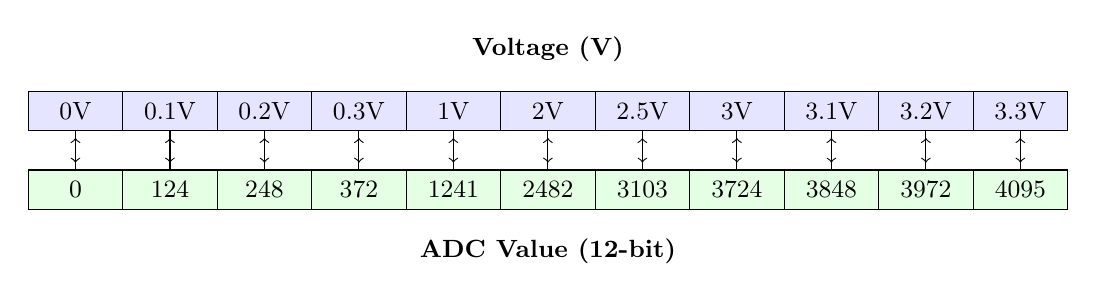
\begin{tikzpicture}[
		every node/.style={font=\small},
		voltage/.style={draw, fill=blue!10, minimum height=0.5cm, minimum width=1.2cm, align=center},
		adc/.style={draw, fill=green!10, minimum height=0.5cm, minimum width=1.2cm, align=center}
		]
		
		% Draw Voltage Levels
		\node[voltage] (v0) at (0, 0) {0V};
		\node[voltage] (v1) at (1.2, 0) {0.1V};
		\node[voltage] (v2) at (2.4, 0) {0.2V};
		\node[voltage] (v3) at (3.6, 0) {0.3V};
		\node[voltage] (v4) at (4.8, 0) {1V};
		\node[voltage] (v5) at (6.0, 0) {2V};
		\node[voltage] (v6) at (7.2, 0) {2.5V};
		\node[voltage] (v7) at (8.4, 0) {3V};
		\node[voltage] (v8) at (9.6, 0) {3.1V};
		\node[voltage] (v9) at (10.8, 0) {3.2V};
		\node[voltage] (v10) at (12.0, 0) {3.3V};
		
		% Draw ADC Values Below Voltage Levels
		\node[adc] (a0) at (0, -1) {0};
		\node[adc] (a1) at (1.2, -1) {124};
		\node[adc] (a2) at (2.4, -1) {248};
		\node[adc] (a3) at (3.6, -1) {372};
		\node[adc] (a4) at (4.8, -1) {1241};
		\node[adc] (a5) at (6.0, -1) {2482};
		\node[adc] (a6) at (7.2, -1) {3103};
		\node[adc] (a7) at (8.4, -1) {3724};
		\node[adc] (a8) at (9.6, -1) {3848};
		\node[adc] (a9) at (10.8, -1) {3972};
		\node[adc] (a10) at (12.0, -1) {4095};
		
		% Add Arrows for Clarity
		\foreach \x in {v0, v1, v2, v3, v4, v5, v6, v7, v8, v9, v10} {
			\draw[->] (\x.south) -- +(0, -0.4);
		}
		\foreach \x in {a0, a1, a2, a3, a4, a5, a6, a7, a8, a9, a10} {
			\draw[->] (\x.north) -- +(0, 0.4);
		}
		
		% Add Axis Label
		\node[above=0.5cm] at (6, 0) {\textbf{Voltage (V)}};
		\node[below=1cm] at (6, -0.5) {\textbf{ADC Value (12-bit)}};
		
	\end{tikzpicture}
	\caption{Mapping of Voltage Levels to ADC Values in the Arduino Nano 33 BLE Sense}
	\label{fig:adc_mapping}
\end{figure}

\subsubsection{Pulse Width Modulation (PWM)}

The Arduino Nano 33 BLE Sense  supports \textbf{Pulse Width Modulation (PWM)} on specific digital pins, enabling the generation of analog-like signals through digital techniques. By rapidly toggling between \textbf{HIGH} and \textbf{LOW} states,\ref{fig:pwm_waveforms} PWM produces a signal with a variable \textbf{duty cycle}, determining the effective voltage output \cite{ArduinoPWM:2024}. Common applications include motor control, LED dimming, and audio tone generation. The \texttt{analogWrite()} function facilitates straightforward PWM implementation.
\\ \\
\vspace{1em} % Adds vertical space (adjust as needed)
\begin{figure}[h!]
	\centering
	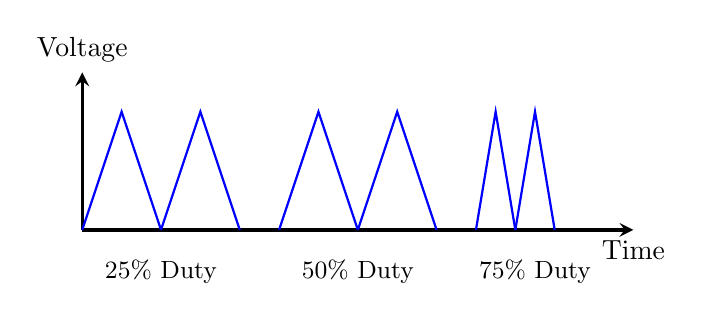
\begin{tikzpicture}[
		axis/.style={very thick, ->, >=stealth},
		wave/.style={thick, draw=blue},
		label/.style={font=\small, anchor=north}
		]
		
		% Draw axes
		\draw[axis] (0, 0) -- (7, 0) node[anchor=north] {Time};
		\draw[axis] (0, 0) -- (0, 2) node[anchor=south] {Voltage};
		
		% Draw PWM waveforms
		% 25% Duty Cycle
		\draw[wave] (0, 0) -- (0.5, 1.5) -- (1, 0);
		\draw[wave] (1, 0) -- (1.5, 1.5) -- (2, 0);
		
		% 50% Duty Cycle
		\draw[wave] (2.5, 0) -- (3, 1.5) -- (3.5, 0);
		\draw[wave] (3.5, 0) -- (4, 1.5) -- (4.5, 0);
		
		% 75% Duty Cycle
		\draw[wave] (5, 0) -- (5.25, 1.5) -- (5.5, 0);
		\draw[wave] (5.5, 0) -- (5.75, 1.5) -- (6, 0);
		
		% Add labels for duty cycles
		\node[label] at (1, -0.25) {25\% Duty};
		\node[label] at (3.5, -0.25) {50\% Duty};
		\node[label] at (5.75, -0.25) {75\% Duty};
		
	\end{tikzpicture}
	\caption{PWM Waveforms with Different Duty Cycles}
	\label{fig:pwm_waveforms}
\end{figure}

\subsubsection{SPI Pins}
The Arduino Nano 33 BLE supports \textbf{SPI (Serial Peripheral Interface) communication}, which facilitates data exchange between the microcontroller and peripheral devices \ref{fig:spi_communication}such as sensors or shift registers \cite{ArduinoSPI:2024}.
\\ \\
\vspace{1em} % Adds vertical space (adjust as needed)
\begin{figure}[h!]
	\centering
	\begin{tikzpicture}[
		device/.style={rectangle, draw, fill=green!20, text centered, minimum width=3cm, minimum height=2.5cm, font=\small\bfseries},
		pin/.style={rectangle, draw, fill=blue!10, minimum width=2cm, minimum height=1cm, align=center, font=\small},
		arrow/.style={->, thick},
		label/.style={font=\small},
		every node/.style={align=center}
		]
		
		% Master Device (Microcontroller)
		\node[device] (master) at (-3, 0) {Microcontroller\\(Master)};
		
		% Slave Device (Peripheral)
		\node[device, fill=red!20] (slave) at (10, 0) {Peripheral Device\\(Slave)};
		
		% Master Pins
		\node[pin, right=2cm of master.north] (sck) {SCK (D13)};
		\node[pin, below=0.5cm of sck] (mosi) {MOSI (D11)};
		\node[pin, below=0.5cm of mosi] (miso) {MISO (D12)};
		\node[pin, below=0.5cm of miso] (ss) {SS (D10)};
		
		% Slave Pins
		\node[pin, left=2cm of slave.north] (sclk_slave) {SCK};
		\node[pin, below=0.5cm of sclk_slave] (sdi) {SDI};
		\node[pin, below=0.5cm of sdi] (sdo) {SDO};
		\node[pin, below=0.5cm of sdo] (cs) {CS};
		
		% Connections
		\draw[arrow] (sck.east) -- (sclk_slave.west) node[midway, above] {Clock (SCLK)};
		\draw[arrow] (mosi.east) -- (sdi.west) node[midway, above] {Data to Slave (SDI)};
		\draw[arrow] (sdo.west) -- (miso.east) node[midway, above] {Data to Master (SDO)};
		\draw[arrow] (ss.east) -- (cs.west) node[midway, above] {Chip Select (CS)};
		
	\end{tikzpicture}
	\caption{SPI Communication between Master and Slave Devices}
	\label{fig:spi_communication}
\end{figure}
\begin{itemize}
	\item \textbf{MISO (Master Input Slave Output):} Receives data from peripherals.
	\item \textbf{MOSI (Master Output Slave Input):} Sends data to peripherals.
\end{itemize}


\subsubsection{I2C Pins}
The board features the \textbf{I2C protocol}, a two-wire communication standard  used for connecting multiple devices. Figure \ref{fig:i2c_communication} demonstrates I2C communication configurations \cite{ArduinoI2C:2024}.
\begin{itemize}
	\item \textbf{MISO (Master Input Slave Output):} Receives data from peripherals. \ref{fig:arduino_master}
	\item \textbf{MOSI (Master Output Slave Input):} Sends data to peripherals.\ref{fig:arduino_slave}
\end{itemize}
\begin{figure}[h!]
	\centering
	% Arduino as Slave
	\begin{subfigure}[b]{0.45\textwidth}
		\centering
		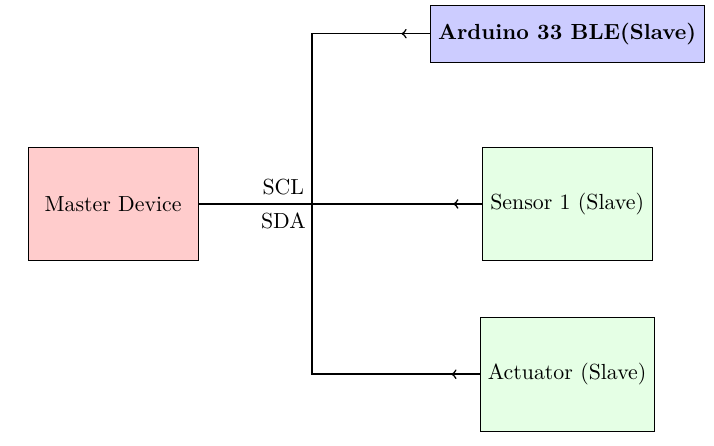
\includegraphics[width=\textwidth]{Images/arduinoSlavei2c.png}
		\caption{Arduino as Slave in I2C Communication}
		\label{fig:arduino_slave}
	\end{subfigure}
	\hfill
	% Arduino as Master
	\begin{subfigure}[b]{0.45\textwidth}
		\centering
		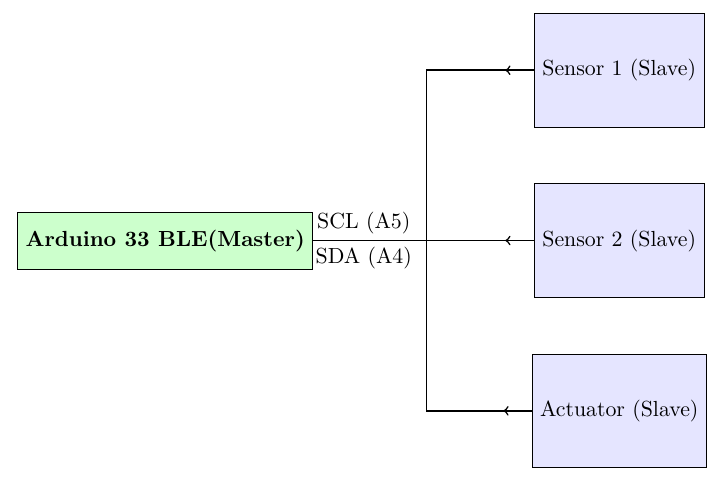
\includegraphics[width=\textwidth]{Images/arduinoMasteri2c.png}
		\caption{Arduino as Master in I2C Communication}
		\label{fig:arduino_master}
	\end{subfigure}
	\caption{I2C Communication with Arduino in Master and Slave Configurations.}
	\label{fig:i2c_communication}
\end{figure}

\begin{itemize}
	\item \textbf{SCL (Serial Clock Line):} Synchronizes data transfer.
	\item \textbf{SDA (Serial Data Line):} Transmits and receives data.
\end{itemize} 





\subsubsection{UART Pins}
The board also includes support for the \textbf{UART (Universal Asynchronous Receiver-Transmitter) protocol}, which enables serial communication. Figure \ref{fig:uart_pin_operation} illustrates UART pin operation.  \cite{BookElectronics:2020}.

\begin{figure}[h!]
	\centering
	\begin{tikzpicture}[
		device/.style={rectangle, draw, fill=blue!20, text centered, minimum width=2cm, minimum height=1cm, font=\tiny},
		pin/.style={rectangle, draw, fill=green!10, text centered, minimum width=0.5cm, minimum height=0.8cm, font=\tiny},
		data/.style={draw, ->, thick},
		label/.style={font=\tiny\bfseries, align=center}
		]
		
		% Microcontroller Node
		\node[device, align=center] (arduino) at (0, 0) {Arduino Nano 33 BLE\\Sense Rev2};
		
		% Rx and Tx Pins
		\node[pin, left=0cm of arduino] (rx) {Rx (D0)};
		\node[pin, right=0cm of arduino] (tx) {Tx (D1)};
		
		% External Device Nodes
		\node[device, align=center] (external_tx) at (-5, 0) {External Device\\(Data Source)};
		\node[device, align=center] (external_rx) at (5, 0) {External Device\\(Data Sink)};
		
		% Data Flow Arrows
		\draw[data] (external_tx.east) -- node[above, font=\scriptsize] {Transmit} (rx.west);
		\draw[data] (tx.east) -- node[above, font=\scriptsize] {Receive} (external_rx.west);
	\end{tikzpicture}
	\caption{UART Pin Operation on Arduino Nano 33 BLE Sense }
	\label{fig:uart_pin_operation}
\end{figure}
\begin{itemize}
	\item \textbf{Rx (Receive):} Used to receive serial data.
	\item \textbf{Tx (Transmit):} Used to send serial data.
\end{itemize}


\subsubsection{External Interrupt Pins}
All \textbf{digital pins} can be configured as \textbf{external interrupt pins}. These are used to pause the main program when an urgent task or event occurs, ensuring immediate response to critical inputs.  \cite{BookElectronics:2020}.

\subsubsection{Special Pins}
The Arduino Nano 33 BLE Sense  includes special pins \ref{fig:special_pins}  that serve unique purposes in various applications. These pins include the built-in LED connected to \textbf{Pin 13} and the \textbf{AREF pin} for analog reference voltage . \cite{BookElectronics:2020}
\begin{itemize}
	
	\item \textbf{LED (Pin 13):} The board features a built-in LED connected to \textbf{pin 13}, often used for debugging or indicating system states.
	\item \textbf{AREF Pin:} The \textbf{Analog Reference (AREF)} pin is used to provide a reference voltage for analog inputs, ensuring precise readings.
\end{itemize}

\begin{figure}[h!]
	\centering
	\begin{tikzpicture}[
		pin/.style={rectangle, draw, fill=green!10, text centered, minimum width=2.5cm, minimum height=1.2cm, font=\small},
		label/.style={font=\small\bfseries},
		arrow/.style={draw, ->, thick, >=stealth},
		node distance=3cm
		]
		
		% Arduino Node
		\node[pin, fill=blue!20] (arduino) at (0, 0) {Arduino Nano 33 BLE Sense };
		
		% LED Pin Node
		\node[pin, right=1cm of arduino] (ledpin) {LED (Pin 13)};
		
		% AREF Pin Node
		\node[pin, above=1cm of arduino] (arefpin) {AREF Pin};
		
		% LED Description
		\node[pin, right=1cm of ledpin] (leddesc) {Built-in LED)};
		
		% AREF Description
		\node[pin, above=1cm of arefpin] (arefdesc) {Analog Reference};
		
		% Arrows
		\draw[arrow] (arduino.east) -- node[above] {} (ledpin.west);
		\draw[arrow] (arduino.north) -- node[left] {} (arefpin.south);
		\draw[arrow] (ledpin.east) -- node[above] {} (leddesc.west);
		\draw[arrow] (arefpin.north) -- node[right] {} (arefdesc.south);
		
	\end{tikzpicture}
	\caption{Special Pins on Arduino Nano 33 BLE Sense }
	\label{fig:special_pins}
\end{figure}

\subsection*{Troubleshooting:}

\begin{itemize}
	\item \textbf{Initialization Failure:} If the message "IMU initialization failed" appears, double-check the board selection and connection.
	\item \textbf{Stuck or Invalid Data:} If accelerometer values don’t change when moving the board, try resetting the board or re-uploading the code\cite{Arduino:2024h}.
\end{itemize}


\subsection*{Further readings}
\begin{itemize}
	\item\textbf{1.	Sensor Fusion Algorithms:} Madgwick filter: Learn about the Madgwick filter, an efficient algorithm for orientation estimation, used widely in wearable and mobile devices\cite{Madgwick:2010}.
	\item\textbf{2.	Inertial Navigation Systems:} o	Explore how IMUs are used in inertial navigation systems for vehicles, drones, and robots, where GPS signals are unavailable or unreliable\cite{Jung:2018}.
	\item\textbf{3.	IMU Calibration Techniques:}o	For further understanding of the calibration process, including advanced techniques like sensor fusion, bias compensation, and drift correction, review the calibration methods used for IMUs in applications such as robotics and aerospace\cite{Oh:2017}.
	
\end{itemize}










